\section{Case Study: The situation in Greece}
We ask participants how they assess the situation in Greece.  We examine Greece in detail for many reasons. Among all borrower countries Greece received by far the 
highest volume of loans and was most severely affected by the European debt crisis. Hence, the crisis in Greece was by far the most salient and widely debated. 
The \textit{aid$&$reform} ignited a large number 
of protests in Greece. Also Greece is the only borrower country which has not yet repaid its loans. Our two questions regarding the situation in Greece are the following. 
In question 6 of our survey we ask, similar to question 4, which party benefited most from loans
to Greece. Again, we expect to find a nation-serving bias between citizens from borrower
and lender countries. One might argue, that 
the resistance of the population in Greece was by far the most salient and the consequences for the population the most drastic. This might lead to a higher level of agreement between borrower and lender countries alike that the lender countries
were the main beneficiaries of the rescue program to Greece causing the divergence in opinions between lender and borrower countries to 
disappear. However, it also seems plausible that there is some level of solidarity between other lender countries and Greece causing 
the divergences to remain largely constant. We ask whether Greece will repay outstanding debt. According to 
our nation-serving hypothesis we would expect citizens from Greece (and potentially other borrower countries) to display a higher degree of confidence 
regarding the repayment of the outstanding level of debt. 

\begin{figure}[h!]
    \centering
    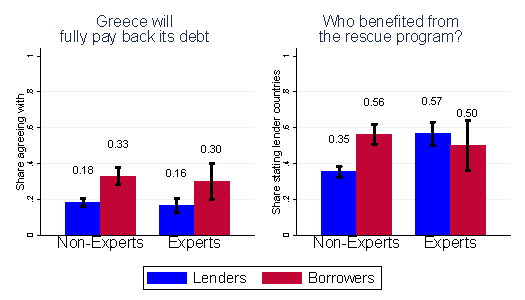
\includegraphics[scale=1.2]{graph6.pdf}
    \caption{Caption}
    \label{fig:my_label}
\end{figure}


The results show that there is substantial divergence about the beneficiaries from the rescue program to Greece in our sample of non-experts. This supports the assumption that there exists some degree of solidarity among citizens of lender countries. 
Participants from lender and borrower countries in the expert and non-expert sample alike show a nation-serving bias when assessing the ability of Greece to repay it's debt. 
 \clearpage
 The results show that experts from  lender countries are 20 percentage points more likely to state that the lender countries were the primary beneficiaries from the loans to Greece. The difference between lender countries and borrower countries is slightly smaller when they are specifically asked about Greece, than when the question is asked more generically. Participants from borrower and lender countries diverge if Greece will be able to fully repay its debt. The observed difference is statistically significant for the sample of citizens and the sample of experts.  
 \\
\begin{figure}[h!] 
\begin{center}
     \caption{Situation in Greece}
     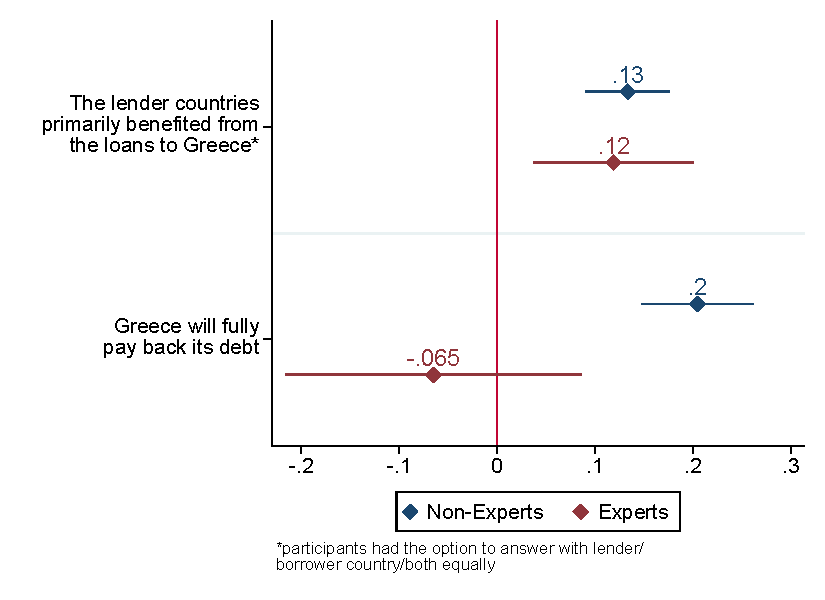
\includegraphics[scale=0.8]{Question6_7_base.pdf}
     \label{fig:my_label}
     \end{center}
     \tiny
     \tablenotes{The exact wording of the question was the following.   Question 6: Who primarily benefited from the loans to Greece; Question 7: Greece will fully pay back it's debt}
\end{figure}